\section{Sch\"{a}r mountain waves test}
\label{sec:cp:schaerWaves}

Chapter~\ref{ch:slanted} assessed a finite volume model of the fully compressible Euler equations with a Lorenz staggering using a test case with a stratified atmosphere initially at rest above an isolated mountain.
We now turn our attention to a transport-dominated test case that presents a challenge to the transport schemes within the dynamical model.
As specified by \citet{schaer2002}, the test prescribes flow over idealised terrain with small-scale and large-scale undulations that induce propagating and evanescent gravity waves.
We use the test to compare results from the two finite volume model variants with Lorenz and generalised Charney--Phillips staggerings against the reference solution from \citet{melvin2010}.

Following \citet{melvin2010}, the domain is \SI{300}{\kilo\meter} wide and \SI{30}{\kilo\meter} high, and the mesh spacing is $\Delta x = \SI{500}{\meter}$ and $\Delta z^\star = \SI{300}{\meter}$.
The mountain profile has the same form as equation~\eqref{eqn:resting:mountain}, but the mountain waves test has a lower peak mountain height of $h_0 = \SI{250}{\meter}$.  As in the resting atmosphere test (section~\ref{sec:slanted:resting}), $a = \SI{5}{\kilo\meter}$ is the mountain half-width and $\lambda = \SI{4}{\kilo\meter}$ is the wavelength.

A uniform horizontal wind $(u, w) = (10, 0)\:\si{\meter\per\second}$ is prescribed in the interior domain and at the inlet boundary.  No normal flow is imposed at the top and bottom boundaries and the velocity field has a zero gradient outlet boundary condition.

The initial thermodynamic conditions have constant static stability with $N = \SI{0.01}{\per\second}$ everywhere such that
\begin{align}
	\theta(z) = \theta_0 \exp \left( \frac{N^2}{g} z \right) \label{eqn:cp:schaerWaves:thermal-profile}
\end{align}
where the temperature at $z=0$ is $\theta_0 = \SI{288}{\kelvin}$.
Potential temperature values are prescribed at the inlet and upper boundary using equation~\eqref{eqn:cp:schaerWaves:thermal-profile}, and a zero gradient boundary condition is applied at the outlet.
At the ground, fixed gradients are imposed by calculating the component of $\nabla \theta$ normal to each face using the vertical derivative of equation~\eqref{eqn:cp:schaerWaves:thermal-profile}.
For the Exner function of pressure, hydrostatic balance is prescribed on top and bottom boundaries and the inlet and outlet are zero normal gradient.

Sponge layers are added to the upper \SI{10}{\kilo\meter} and leftmost \SI{10}{\kilo\meter} at the inlet boundary to damp the reflection of waves.
The damping term \(\mu\) in the momentum equation \eqref{eqn:exnerFoam:momentum} is a function adapted from \citet{melvin2010} such that
\begin{subequations}
\begin{align}
	\mu(x, z) &= \mu_\mathrm{upper} + \mu_\mathrm{inlet} \\
	\mu_\mathrm{upper}(z) &= \begin{cases}
		\overline{\mu} \sin^2 \left( \frac{\pi}{2} \frac{z - z_B}{H - z_B} \right) & \enskip \text{if $z \geq z_B$,} \\
		0 & \enskip \text{otherwise,} \\
	\end{cases} \\
	\mu_\mathrm{inlet}(x) &= \begin{cases}
		\overline{\mu} \sin^2 \left( \frac{\pi}{2} \frac{x_I - x}{x_I - x_0} \right) & \enskip \text{if $x < x_I$,} \\
		0 & \enskip \text{otherwise,}
	\end{cases}
\end{align}%
\end{subequations}
where $\overline{\mu} = \SI{1.2}{\per\second}$ is the damping coefficient, $z_B = \SI{20}{\kilo\meter}$ is the bottom of the sponge layer, $H = \SI{30}{\kilo\meter}$ is the top of the domain, $x_0 = \SI{-150}{\kilo\meter}$ is the leftmost limit of the domain and $x_I = \SI{-140}{\kilo\meter}$ is the rightmost extent of the inlet sponge layer.
The sponge layer is only active on faces whose normal is vertical so that it damps vertical momentum only.
Note that, while the domain itself is \SI{30}{\kilo\meter} in height, for the purposes of generating BTF meshes, the domain height is set to \SI{20}{\kilo\meter} because the sponge layer occupies the uppermost \SI{10}{\kilo\meter}.

\begin{figure}
	\centering
	\begin{subfigure}{0.55\textwidth}
		\centering
		\caption{Lorenz staggering, linearUpwind transport}
		\label{fig:cp:schaerWaves:w:linearUpwind}
		\includegraphics{thesis/cp/schaerWaves/fig-btf-300dz-linearUpwind-w.pdf}
	\end{subfigure}
	\begin{subfigure}{0.44\textwidth}
		\centering
		\caption{Lorenz staggering, cubicFit transport}
		\label{fig:cp:schaerWaves:w:cubicFit}
		\includegraphics{thesis/cp/schaerWaves/fig-btf-300dz-cubicFit-w.pdf}
	\end{subfigure}
	\\
	\vspace*{1em}
	%
	\begin{subfigure}{0.55\textwidth}
		\centering
		\caption{Generalised Charney--Phillips staggering}
		\label{fig:cp:schaerWaves:w:cp}
		\includegraphics{thesis/cp/schaerWaves/fig-btf-300dz-cp-w.pdf}
	\end{subfigure}
	\begin{subfigure}{0.44\textwidth}
		\centering
		\caption{Reference solution by \citet{melvin2010}}
		\label{fig:cp:schaerWaves:w:melvin}
		\raisebox{0.2in}{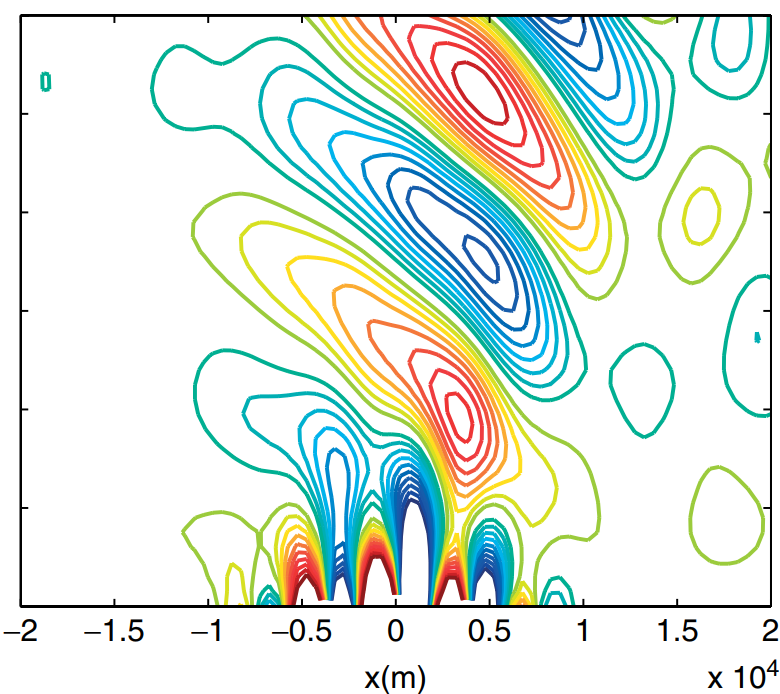
\includegraphics[height=1.9in]{cp/schaerWaves/melvin2010-w-mass-conserving-sisl.png}}
	\end{subfigure}
	\caption{Vertical velocities at the end of integration of the Sch\"{a}r mountain waves test case.
	Results obtained using a BTF mesh and Lorenz staggering, with potential temperature and momentum transported by (\subcaptionref{fig:cp:schaerWaves:w:linearUpwind}) the linearUpwind scheme and
	(\subcaptionref{fig:cp:schaerWaves:w:cubicFit}) the cubicFit scheme, and (\subcaptionref{fig:cp:schaerWaves:w:cp}) using a BTF mesh and generalised Charney--Phillips staggering.
	For comparison, (\subcaptionref{fig:cp:schaerWaves:w:melvin}) provides a reference solution obtained with a mass-conserving semi-implicit semi-Lagrangian model \citep{melvin2010}.
	Contours are plotted every \SI{0.05}{\meter\per\second}.  In figures (\subcaptionref{fig:cp:schaerWaves:w:linearUpwind}), (\subcaptionref{fig:cp:schaerWaves:w:cubicFit}) and (\subcaptionref{fig:cp:schaerWaves:w:cp}), ascending velocities are marked by solid black lines and descending velocities are marked by dashed red lines.
Only the lowest \SI{12}{\kilo\meter} in the central region of the domain is shown.  The entire domain is \SI{300}{\kilo\meter} wide and \SI{30}{\kilo\meter} high.
	}
	\label{fig:cp:schaerWaves:w}
\end{figure}

The test is integrated forward by five hours using a time-step of \SI{8}{\second}.  At the end of the simulation, gravity waves are apparent in the contours of vertical velocity (figure~\ref{fig:cp:schaerWaves:w}).
Results are presented for the Lorenz model variant, with momentum and potential temperature being transported using the linearUpwind scheme (figure~\ref{fig:cp:schaerWaves:w:linearUpwind}) and the cubicFit scheme (figure~\ref{fig:cp:schaerWaves:w:cubicFit}), and for the generalised Charney--Phillips model variant (figure~\ref{fig:cp:schaerWaves:w:cp}), and all are in general agreement with the reference solution from \citet{melvin2010}, reproduced in figure~\ref{fig:cp:schaerWaves:w:melvin}.
All four results presented in figure~\ref{fig:cp:schaerWaves:w} were all obtained using the same BTF mesh.

Spurious distortions are visible in the vertical velocity contours using the Lorenz model variant and the linearUpwind transport scheme (figure~\ref{fig:cp:schaerWaves:w:linearUpwind}), and similar error structures have been found in previous studies that were attributed to numerical errors associated with BTF mesh distortions \citep{schaer2002,klemp2003}.
In agreement with these previous findings, we find that spurious gravity wave distortions can be avoided by switching from a BTF mesh to a slanted cell mesh or cut cell mesh (results not shown).
We also find that spurious gravity wave distortions can be avoided by transporting momentum and potential temperature on a BTF mesh using the cubicFit scheme (figure~\ref{fig:cp:schaerWaves:w:cubicFit}).
Avoiding such spurious gravity waves distortions using either approach produces solutions that closely match the reference solution (figure~\ref{fig:cp:schaerWaves:w:melvin}).
Given these results, we can attribute spurious gravity wave distortions to transport scheme errors associated with flow that is misaligned with mesh layers.
Unlike the results obtained by \citet{shaw-weller2016} that used an older formulation of the cubicFit scheme, potential temperature errors are negligible for all types of mesh when using the most recent formulation of the cubicFit scheme documented in chapter~\ref{ch:cubicFit}.

As seen in figure~\ref{fig:cp:schaerWaves:w:cp}, the generalised Charney--Phillips model variant produces gravity waves with spurious distorted structures similar to those obtained using the Lorenz model variant with the linearUpwind scheme (figure~\ref{fig:cp:schaerWaves:w:linearUpwind}).
In addition, as evidenced by the density of vertical velocity contour lines in figure~\ref{fig:cp:schaerWaves:w:cp}, the generalised Charney--Phillips model variant produces gravity wave amplitudes that are too large compared to the reference solution.

\TODO{This is not a summary of the results presented...}
In summary, accurate gravity wave solutions were obtained using the Lorenz model variant with cut cell meshes and slanted cell meshes, and accurate solutions were also obtained by transporting momentum and potential temperature on the BTF mesh using the cubicFit scheme.
A less accurate solution was obtained on the BTF mesh using the generalised Charney--Phillips model variant, but all results were in general agreement with the reference solution from \citet{melvin2010}.
Knowing that an improved transport scheme was responsible for the improved gravity wave solution using the Lorenz model variant, we conjecture that the generalised Charney--Phillips model variant produces less accurate results because the model uses a transport scheme that is insufficiently accurate.
In the next section we perform a further comparison between Lorenz and generalised Charney--Phillips model variants using a new test case to excite the Lorenz computational mode.

\TODO{Would it be worth showing that the CP model can produce the correct result by using a smoother terrain-following mesh?}
